% Provenance (never printed): see sources/outline_sources.md (Year 1:
% the Solar System, planetology). Kepler's laws, the moment of inertia and
% the Stefan--Boltzmann law are owned by the physics series and recalled
% here; the equilibrium temperature and the Bond albedo are re-founded from
% Book 2 grade 10. Curves computed in figdata/bachelor-1/planet_table.py;
% numbers of the exercises and problem in the Book 3 scratch calculator
% ch03.py.
\chapter{Planetología comparada}\label{ch:b1:comparative-planetology}

Venus y la Tierra son casi gemelas: Venus tiene el \qty{95}{\percent} del radio terrestre y
el \qty{81}{\percent} de su masa. Sin embargo, la Tierra tiene océanos, una atmósfera de
nitrógeno y oxígeno y placas en movimiento, mientras que Venus se oculta bajo nubes, con una
superficie a \qty{737}{K}, más caliente que cualquier horno de cocina, aplastada por una
atmósfera de dióxido de carbono a \qty{92}{bar}. Marte, la mitad de grande que la Tierra,
tiene una atmósfera fría y tenue, volcanes gigantes y cañones, pero no placas en movimiento.
Más allá, Júpiter y Saturno están formados sobre todo por hidrógeno y helio; Urano y Neptuno,
sobre todo por los hielos de agua, metano y amoníaco. Comparar los planetas es la única manera
de poner a prueba lo que creemos saber de la Tierra: por qué su interior está estratificado,
por qué su clima es suave, por qué solo ella tiene tectónica de placas. Este capítulo pesa y
mide los planetas, lee sus interiores a partir de sus densidades y del modo en que se reparte
su masa, compara sus temperaturas y atmósferas, y termina con las lunas y los cuerpos
pequeños que conservan el registro de la juventud del sistema solar.
% ledger: nasa:venus, earth:Rmean, earth:mass, nasa:uranus-structure

\begin{recall}
Los planetas giran alrededor del Sol en elipses, y el cuadrado del periodo de un satélite es
proporcional al cubo de su semieje mayor (tercera ley de Kepler, en el libro de física de
primer año, donde también se define el momento de inercia de un sólido; una esfera uniforme
tiene $I = \tfrac25MR^2$). Un cuerpo negro radia $\sigma T^4$ por unidad de área (libro de
física de segundo año). El sistema solar y sus planetas rocosos y gigantes se describieron en
el libro 1 (año 6); el albedo y la \omterm{def:b1:comparative-planetology:equilibrium-temperature}{temperatura de equilibrio} de un planeta se vieron en el
libro 2 (año 10), y el efecto invernadero, en el libro 1 (año 9).
\end{recall}

\begin{omfigure}
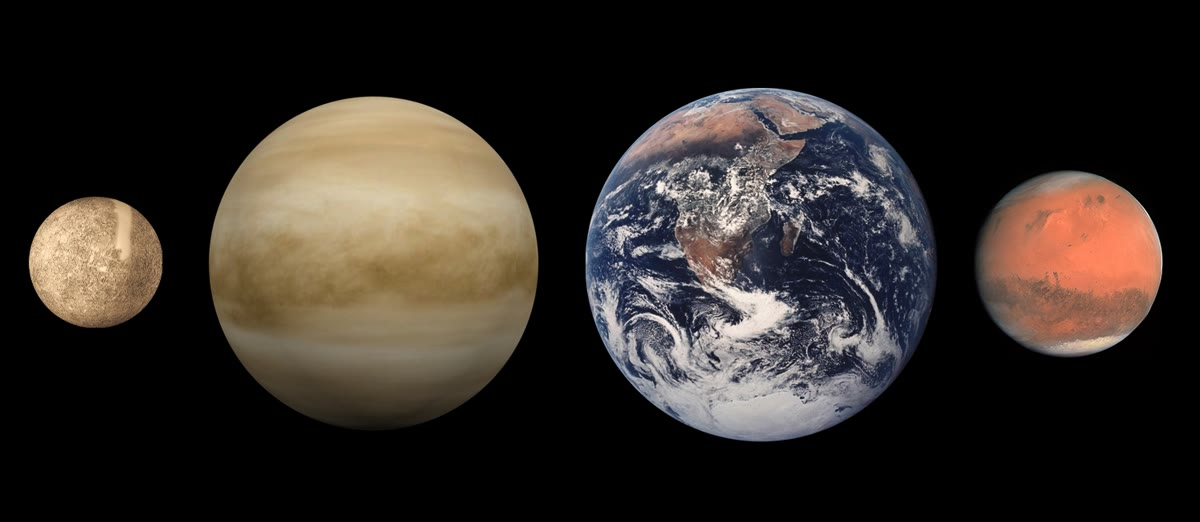
\includegraphics[width=0.85\linewidth]{images/book3/b1-terrestrial-planet-sizes.jpg}

{\small Los cuatro \omterm{def:b1:comparative-planetology:planet-types}{planetas terrestres} a escala, de izquierda a derecha Mercurio, Venus, la
Tierra y Marte (distancias no a escala; Venus vista con luz visible, con su superficie oculta
bajo las nubes). NASA, dominio público.}
% ledger: commons:terrestrial-sizes
\end{omfigure}

\section{Pesar y medir los planetas}

El radio de un planeta se mide a partir de su diámetro angular y de su distancia, o, para un
planeta visitado por naves espaciales, mediante altimetría por radar y por láser. Su masa es
más difícil: solo se percibe por la gravedad que el planeta ejerce sobre otra cosa.

\begin{method}[Masa de un planeta a partir de la órbita de un satélite]\label{met:b1:comparative-planetology:mass}
Para un satélite de masa despreciable, en una órbita casi circular de radio (semieje mayor)
$a$ y periodo sidéreo $T$ alrededor de un planeta de masa $M$:
\begin{enumerate}
  \item conviértanse $a$ a metros y $T$ a segundos;
  \item la tercera ley de Kepler da $GM = 4\pi^2a^3/T^2$: este producto es lo que mide la
        órbita, con una precisión mucho mayor que la de $G$ por sí sola;
  \item divídase por $G = \qty{6.6743e-11}{m^3.kg^{-1}.s^{-2}}$ para obtener $M$.
\end{enumerate}
Un planeta sin luna (Mercurio, Venus) se pesa de la misma manera, a partir de la órbita o de la
desviación de una nave que pasa cerca de él.
\end{method}

\begin{example}
Ío, la mayor de las lunas interiores de Júpiter, orbita a $a = \qty{421.8e3}{km}$ en
\num{1.769138} días, es decir, $T = \qty{152854}{s}$. Entonces
\[
  GM = \frac{4\pi^2\times(\qty{4.218e8}{m})^3}{(\qty{152854}{s})^2}
  = \qty{1.268e17}{m^3.s^{-2}}, \qquad
  M = \frac{\num{1.268e17}}{\num{6.6743e-11}} = \qty{1.900e27}{kg},
\]
que concuerda con la masa tabulada de Júpiter, \qty{1.898e27}{kg}, con un error del
\qty{0.1}{\percent}. La masa de Ío, \num{4.7e-5} de la de Júpiter, es despreciable; el pequeño
exceso procede del abultamiento ecuatorial de Júpiter, que atrae a una luna cercana algo más
fuerte de lo que lo haría una esfera de la misma masa.
% ledger: nasa:io, nasa:jupiter, const:G
\end{example}

Con la masa y el radio se obtiene la densidad media $\bar\rho =
3M/(4\pi R^3)$, la primera pista sobre de qué está hecho un planeta. Las densidades de los
planetas se agrupan en dos grupos (véase la figura siguiente): Mercurio, Venus, la Tierra y
Marte están entre unos \num{3900} y \qty{5500}{kg.m^{-3}}, más densos que cualquier roca
común; los cuatro planetas exteriores están entre \num{690} y \qty{1640}{kg.m^{-3}}, cerca de
la densidad del agua, y Saturno incluso por debajo de ella.
% ledger: planet:Mercury.density, planet:Mars.density, planet:Earth.density, planet:Saturn.density, planet:Neptune.density

\begin{omfigure}
\begin{tikzpicture}
\begin{axis}[omrecord, width=0.86\linewidth, height=6.2cm, xmode=log,
  xmin=800, xmax=150000, ymin=0, ymax=6300, xlabel={radio ecuatorial (km)},
  ylabel={densidad media (\unit{kg.m^{-3}})}, tick label style={font=\scriptsize},
  label style={font=\small}]
\addplot[only marks, mark=*, mark size=2.4pt, brown!70!black] table[x=R_km, y=density,
  restrict expr to domain={\thisrow{idx}}{0:2}] {figdata/out/bachelor-1-planet_table-bodies.dat};
\addplot[only marks, mark=*, mark size=2.4pt, brown!70!black] table[x=R_km, y=density,
  restrict expr to domain={\thisrow{idx}}{4:4}] {figdata/out/bachelor-1-planet_table-bodies.dat};
\addplot[only marks, mark=*, mark size=2.4pt, orange!85!black] table[x=R_km, y=density,
  restrict expr to domain={\thisrow{idx}}{5:6}] {figdata/out/bachelor-1-planet_table-bodies.dat};
\addplot[only marks, mark=*, mark size=2.4pt, omDef] table[x=R_km, y=density,
  restrict expr to domain={\thisrow{idx}}{7:8}] {figdata/out/bachelor-1-planet_table-bodies.dat};
\addplot[only marks, mark=o, mark size=2.4pt, black!60] table[x=R_km, y=density,
  restrict expr to domain={\thisrow{idx}}{3:3}] {figdata/out/bachelor-1-planet_table-bodies.dat};
\addplot[only marks, mark=o, mark size=2.4pt, black!60] table[x=R_km, y=density,
  restrict expr to domain={\thisrow{idx}}{9:9}] {figdata/out/bachelor-1-planet_table-bodies.dat};
\addplot[black!40, densely dashed] coordinates {(800,1000) (150000,1000)};
\begin{scope}[font=\scriptsize]
\node[left] at (axis cs:2439.5,5429) {Mercurio};
\node[below left] at (axis cs:6052,5243) {Venus};
\node[above] at (axis cs:6378,5514) {Tierra};
\node[left] at (axis cs:3396,3934) {Marte};
\node[left] at (axis cs:1737.5,3340) {Luna};
\node[right] at (axis cs:1188,1850) {Plutón};
\node[above] at (axis cs:71492,1326) {Júpiter};
\node[left] at (axis cs:60268,687) {Saturno};
\node[right] at (axis cs:25559,1270) {Urano};
\node[above] at (axis cs:24764,1638) {Neptuno};
\node[above left, black!60] at (axis cs:150000,1000) {agua};
\end{scope}
\end{axis}
\end{tikzpicture}

{\small Densidad media frente al radio (logarítmico) de los ocho planetas (rellenos:
terrestres, \omterm{def:b1:comparative-planetology:planet-types}{gigantes gaseosos} y \omterm{def:b1:comparative-planetology:planet-types}{gigantes de hielo}), de la Luna y de Plutón (círculos vacíos).
Datos de la hoja de datos planetarios de la NASA.}
% ledger: planet:Mercury.diameter, planet:Venus.diameter, planet:Earth.diameter, planet:Moon.diameter, planet:Mars.diameter, planet:Jupiter.diameter, planet:Saturn.diameter, planet:Uranus.diameter, planet:Neptune.diameter, planet:Pluto.diameter, planet:Mercury.density, planet:Venus.density, planet:Earth.density, planet:Moon.density, planet:Mars.density, planet:Jupiter.density, planet:Saturn.density, planet:Uranus.density, planet:Neptune.density, planet:Pluto.density
\end{omfigure}

La densidad media por sí sola no puede distinguir un planeta hecho de un solo material denso
de otro con un centro muy denso y una envoltura más ligera. Un segundo número sí lo hace: cómo
se reparte la masa entre el centro y la superficie.

\begin{definition}[Factor de momento de inercia]\label{def:b1:comparative-planetology:moi}
El \emph{factor de momento de inercia}\index{factor de momento de inercia} de un planeta es el
número
\[
  C = \frac{I}{MR^2} ,
\]
donde $I$ es su momento de inercia respecto de su eje de rotación, $M$ su masa y $R$ su radio
medio. Una esfera uniforme tiene $C = \tfrac25 = 0.4$; un planeta cuya densidad aumenta hacia
el centro tiene $C < 0.4$, tanto menor cuanto más concentrada esté la masa.
\end{definition}

El momento de inercia se mide a partir de la lenta precesión del eje de rotación bajo la
atracción del Sol, junto con el aplanamiento del campo gravitatorio del planeta. Los valores son
reveladores: la Luna, con $C = 0.394$, es casi uniforme; Marte, con $0.366$, y la Tierra, con
$0.3308$, están claramente estratificados; Júpiter, con $0.254$, y Saturno, con $0.210$, tienen
la mayor parte de su masa concentrada hacia el centro.
% ledger: nasa:moon, nasa:mars, earth:MoI, nasa:jupiter, nasa:saturn

\section{De qué están hechos los planetas}

\begin{definition}[Planetas terrestres y gigantes]\label{def:b1:comparative-planetology:planet-types}
Un \emph{planeta terrestre}\index{planeta terrestre} es un planeta formado sobre todo por roca
silicatada y hierro, con superficie sólida: Mercurio, Venus, la Tierra y Marte. Un
\emph{planeta gigante}\index{planeta gigante} es un planeta muchas veces más masivo que la
Tierra, formado sobre todo por elementos ligeros y sus compuestos, y sin superficie sólida. Un
\emph{gigante gaseoso}\index{gigante gaseoso} es un planeta gigante formado sobre todo por
hidrógeno y helio: Júpiter y Saturno. Un \emph{gigante de hielo}\index{gigante de hielo} es un
planeta gigante formado sobre todo por los compuestos que los astrónomos llaman hielos --- agua,
metano y amoníaco ---, bajo una envoltura de hidrógeno y helio: Urano y Neptuno.
\end{definition}

Las atmósferas que miden las sondas y los telescopios confirman la división. La de Júpiter tiene
un \qty{89.8}{\percent} de hidrógeno y un \qty{10.2}{\percent} de helio en volumen; la de
Saturno, un \qty{96.3}{\percent} y un \qty{3.25}{\percent}; en Urano, al menos el
\qty{80}{\percent} de la masa es un fluido caliente y denso de agua, metano y amoníaco sobre un
pequeño núcleo rocoso. La densidad media de un \omterm{def:b1:comparative-planetology:planet-types}{gigante gaseoso} sigue siendo baja aunque su
centro esté muy comprimido, porque el hidrógeno es el elemento más ligero; un \omterm{def:b1:comparative-planetology:planet-types}{gigante de hielo}
es más denso que Saturno porque sus hielos pesan más que el hidrógeno.
% ledger: nasa:jupiter, nasa:saturn, nasa:uranus-structure

Los \omterm{def:b1:comparative-planetology:planet-types}{planetas terrestres} están estratificados como la Tierra: un núcleo rico en hierro bajo un
manto silicatado y una corteza delgada. El modelo más sencillo que usa los dos números medidos,
la densidad media y el \omterm{def:b1:comparative-planetology:moi}{factor de momento de inercia}, tiene dos capas.

\begin{proposition}[El planeta de dos capas]\label{prop:b1:comparative-planetology:two-layer}
Modelicemos un planeta de radio $R$ como un núcleo de radio $xR$ y densidad uniforme $\rho_c$
en el interior de un manto de densidad uniforme $\rho_m$. Su densidad media y su \omterm{def:b1:comparative-planetology:moi}{factor de
momento de inercia} son
\[
  \bar\rho = \rho_m + (\rho_c - \rho_m)\,x^3 , \qquad
  C = \frac25\,\frac{\rho_m + (\rho_c - \rho_m)\,x^5}{\bar\rho} .
\]
Dados $\bar\rho$, $C$ y una densidad supuesta del manto, $\rho_m$, el radio relativo del núcleo
se obtiene de:
\[
  x^2 = \frac{\tfrac52C\bar\rho - \rho_m}{\bar\rho - \rho_m} ,
  \qquad \rho_c = \rho_m + \frac{\bar\rho - \rho_m}{x^3} .
\]
\end{proposition}

\begin{proof}
El planeta es una esfera uniforme de densidad $\rho_m$ y radio $R$ más una esfera de radio $xR$
con el exceso de densidad $\rho_c - \rho_m$. Las masas se suman: $M = \tfrac43\pi R^3[\rho_m + (\rho_c - \rho_m)x^3]$, y dividiendo por el volumen se obtiene $\bar\rho$. Los momentos de inercia
respecto del mismo eje también se suman; una esfera uniforme de densidad $\rho$ y radio $r$ tiene
$I = \tfrac25\cdot\tfrac43\pi\rho r^3\cdot r^2 = \tfrac{8\pi}{15}\rho r^5$, así que
$I = \tfrac{8\pi}{15}R^5[\rho_m + (\rho_c - \rho_m)x^5]$. Dividiendo por
$MR^2 = \tfrac43\pi\bar\rho R^5$ se obtiene $C$. Por último, las dos ecuaciones se leen
$(\rho_c - \rho_m)x^3 = \bar\rho - \rho_m$ y $(\rho_c - \rho_m)x^5 =
\tfrac52C\bar\rho - \rho_m$; dividiendo la segunda por la primera se obtiene $x^2$, y la primera
da $\rho_c$.
\end{proof}

El modelo tiene tres incógnitas y dos datos, así que una de ellas, la densidad del manto, debe
suponerse a partir de lo que pesan bajo presión las rocas de la composición adecuada. La
respuesta es sensible a esa elección cuando $C$ está cerca de $0.4$, porque
$\tfrac52C\bar\rho - \rho_m$ es entonces una pequeña diferencia de números grandes
(\cref{exo:b1:comparative-planetology:10} y el problema). El modelo también ignora la compresión
del manto por su propio peso, que en un planeta tan grande como la Tierra eleva la densidad del
manto profundo muy por encima de la de las rocas superficiales; para la Tierra, la sismología lo
hace mucho mejor (\cref{ch:b1:layered-earth}). Sismómetros colocados en Marte han hecho ahora lo
mismo para ese planeta: donde la tabla planetaria da un radio del núcleo de \qty{1830}{km},
los resultados recientes indican solo entre \qty{1650}{km} y \qty{1675}{km}.
% ledger: nasa:mars-core

\begin{omfigure}
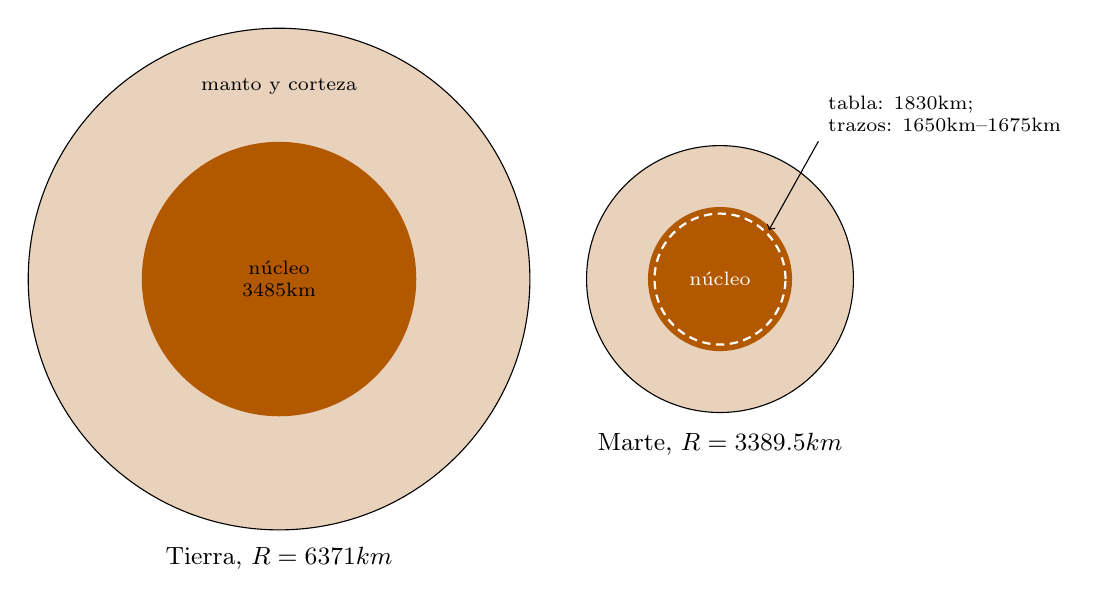
\begin{tikzpicture}[font=\scriptsize]
% scale: 0.5 cm per 1000 km
\fill[brown!35] (0,0) circle (3.1855cm);
\fill[orange!70!black] (0,0) circle (1.7425cm);
\draw (0,0) circle (3.1855cm);
\node[align=center] at (0,0) {núcleo\\ \qty{3485}{km}};
\node[align=center] at (0,2.45) {manto y corteza};
\node at (0,-3.55) {\small Tierra, $R = \qty{6371}{km}$};
\begin{scope}[xshift=5.6cm]
\fill[brown!35] (0,0) circle (1.6948cm);
\fill[orange!70!black] (0,0) circle (0.915cm);
\draw[white, densely dashed, thick] (0,0) circle (0.8313cm);
\draw (0,0) circle (1.6948cm);
\node[align=center, white] at (0,0) {núcleo};
\node at (0,-2.1) {\small Marte, $R = \qty{3389.5}{km}$};
\draw[->] (1.25,1.75) node[above right, align=left] {tabla: \qty{1830}{km};\\ trazos: \qty{1650}{km}--\qty{1675}{km}} -- (0.62,0.62);
\end{scope}
\end{tikzpicture}

{\small La Tierra y Marte a escala, con sus núcleos. En Marte, el borde sólido es el radio del
núcleo de la tabla planetaria, y el círculo de trazos, el radio menor que indican los resultados
sísmicos recientes. Ambos núcleos son ricos en hierro; el de la Tierra tiene una parte interna
sólida, que no se dibuja.}
% ledger: earth:Rmean, earth:Rcore, nasa:mars, nasa:mars-core
\end{omfigure}

\section{Atmósferas y superficies}

La temperatura de un planeta la fija primero la luz solar que absorbe. La irradiancia $S$ a su
distancia $d$ del Sol decrece como $1/d^2$ (\cref{prop:b1:observing-the-sky:inverse-square}):
\qty{1361}{W.m^{-2}} en la Tierra, \qty{2601}{W.m^{-2}} en Venus, \qty{586}{W.m^{-2}} en Marte,
\qty{50}{W.m^{-2}} en Júpiter. Una parte se refleja de inmediato.
% ledger: earth:TSI, nasa:venus, nasa:mars, nasa:jupiter

\begin{definition}[Albedo de Bond]\label{def:b1:comparative-planetology:albedo}
El \emph{albedo de Bond}\index{albedo de Bond} $A$ de un planeta es la fracción de la potencia
total de la luz solar que cae sobre él que refleja y dispersa de vuelta al espacio, en todas las
longitudes de onda y en todas las direcciones.
\end{definition}

La nieve fresca y las nubes brillantes reflejan mucho; la roca oscura y el mar abierto, poco.
Venus, envuelta en nubes brillantes, tiene $A = 0.77$; la Tierra, $0.294$; Marte, $0.250$; la
Luna, roca gris oscura, $0.11$.
% ledger: nasa:venus, earth:albedo, nasa:mars, nasa:moon

\begin{definition}[Temperatura de equilibrio]\label{def:b1:comparative-planetology:equilibrium-temperature}
La \emph{temperatura de equilibrio}\index{temperatura de equilibrio} $T_\mathrm{eq}$ de un planeta
es la temperatura uniforme a la que un cuerpo negro del tamaño del planeta radiaría al espacio
exactamente la potencia que el planeta absorbe del Sol.
\end{definition}

\begin{proposition}[Temperatura de equilibrio]\label{prop:b1:comparative-planetology:teq}
Un planeta de \omterm{def:b1:comparative-planetology:albedo}{albedo de Bond} $A$ que recibe la irradiancia $S$ tiene
\[
  T_\mathrm{eq} = \left(\frac{S(1 - A)}{4\sigma}\right)^{1/4},
  \qquad \sigma = \qty{5.6704e-8}{W.m^{-2}.K^{-4}} .
\]
\end{proposition}

\begin{proof}
El planeta intercepta la luz solar que cae sobre su sección transversal, un disco de área
$\pi R^2$, y absorbe la fracción $1 - A$: absorbe $S(1 - A)\pi
R^2$. Un cuerpo negro (ley de
Stefan--Boltzmann, que se toma del libro de física de segundo año) a temperatura uniforme $T$
radia $\sigma T^4$ desde cada metro cuadrado de su superficie entera, $4\pi R^2$. Igualando las
dos potencias, $4\pi R^2\sigma T^4 = S(1 - A)\pi R^2$, y el factor 4 es el cociente entre el área
de la esfera y su sección transversal.
\end{proof}

Con los valores anteriores, $T_\mathrm{eq}$ es de \qty{255}{K} para la Tierra,
\qty{227}{K} para Venus, \qty{210}{K} para Marte y \qty{270}{K} para la Luna. Venus, aunque
está más cerca del Sol, sale más fría que la Tierra: sus nubes reflejan tres cuartas partes
de la luz solar. La figura siguiente pone estos valores junto a las temperaturas superficiales
medias medidas. Las diferencias son el efecto invernadero, que los párrafos siguientes y los
capítulos sobre el clima (\cref{ch:b1:radiation-heat-transport}) hacen cuantitativo: unos
\qty{33}{K} en la Tierra, unos \qty{510}{K} en Venus y solo unos \qty{4}{K} en Marte.
% ledger: const:sigma, earth:Tsurf, nasa:venus, nasa:mars, planet:Moon.Tmean

\begin{omfigure}
\begin{tikzpicture}
\begin{axis}[ybar, bar width=12pt, width=0.72\linewidth, height=5.8cm,
  ymin=0, ymax=820, xmin=-0.6, xmax=3.6, xtick={0,1,2,3},
  xticklabels={Luna, Marte, Tierra, Venus}, ylabel={temperatura (K)},
  tick label style={font=\scriptsize}, label style={font=\small},
  ymajorgrids, grid style={black!12}, axis lines*=left,
  legend style={font=\scriptsize, at={(0.03,0.97)}, anchor=north west, draw=none},
  nodes near coords, nodes near coords style={font=\tiny},
  every node near coord/.append style={/pgf/number format/fixed, /pgf/number format/precision=0}]
\addplot[fill=omDef!55, draw=omDef] table[x=idx, y=Teq] {figdata/out/bachelor-1-planet_table-temps.dat};
\addplot[fill=omThm!60, draw=omThm] table[x=idx, y=Tsurf] {figdata/out/bachelor-1-planet_table-temps.dat};
\legend{temperatura de equilibrio, temperatura superficial media}
\end{axis}
\end{tikzpicture}

{\small \omterm{def:b1:comparative-planetology:equilibrium-temperature}{Temperatura de equilibrio} (calculada a partir de la irradiancia y del \omterm{def:b1:comparative-planetology:albedo}{albedo de Bond})
y temperatura superficial media medida de cuatro cuerpos. La atmósfera calienta la Tierra y,
sobre todo, Venus; la delgada atmósfera de Marte hace poco; la Luna, sin atmósfera, es en
promedio más fría que su \omterm{def:b1:comparative-planetology:equilibrium-temperature}{temperatura de equilibrio}.}
% ledger: nasa:moon, nasa:mars, earth:TSI, earth:albedo, earth:Tsurf, nasa:venus, planet:Moon.Tmean, const:sigma
\end{omfigure}

La temperatura media de la Luna, unos \qty{253}{K}, queda por debajo de su \omterm{def:b1:comparative-planetology:equilibrium-temperature}{temperatura de
equilibrio}. No es una paradoja: sin atmósfera ni océano que transporten el calor, la cara
diurna está muy caliente y la nocturna muy fría, y como la emisión crece como $T^4$, un cuerpo
con temperaturas desiguales radia la potencia absorbida con una temperatura media más baja que
uno uniforme (\cref{exo:b1:comparative-planetology:11}).

Una atmósfera hace dos cosas: deja pasar la mayor parte de la luz solar y absorbe parte del
infrarrojo que emite el suelo, reemitiendo una parte hacia abajo. Cuánto calienta la superficie
depende de cuánto gas absorbente hay encima de cada metro cuadrado. La presión superficial mide
exactamente eso: $p = mg$ para una columna de masa $m$ por metro cuadrado. La atmósfera de Venus,
a \qty{92}{bar}, es un \qty{96.5}{\percent} de dióxido de carbono; la de Marte, de solo
\qty{6.36}{mbar} de media, es también un \qty{95.1}{\percent} de dióxido de carbono, pero tiene
unas sesenta veces menos gas sobre cada metro cuadrado que la de la Tierra, y muy poco vapor de
agua. Ambos planetas tienen atmósferas de dióxido de carbono; solo una de ellas es espesa.
% ledger: nasa:venus, nasa:mars, earth:psurf

\begin{omfigure}
\begin{minipage}{0.4\linewidth}
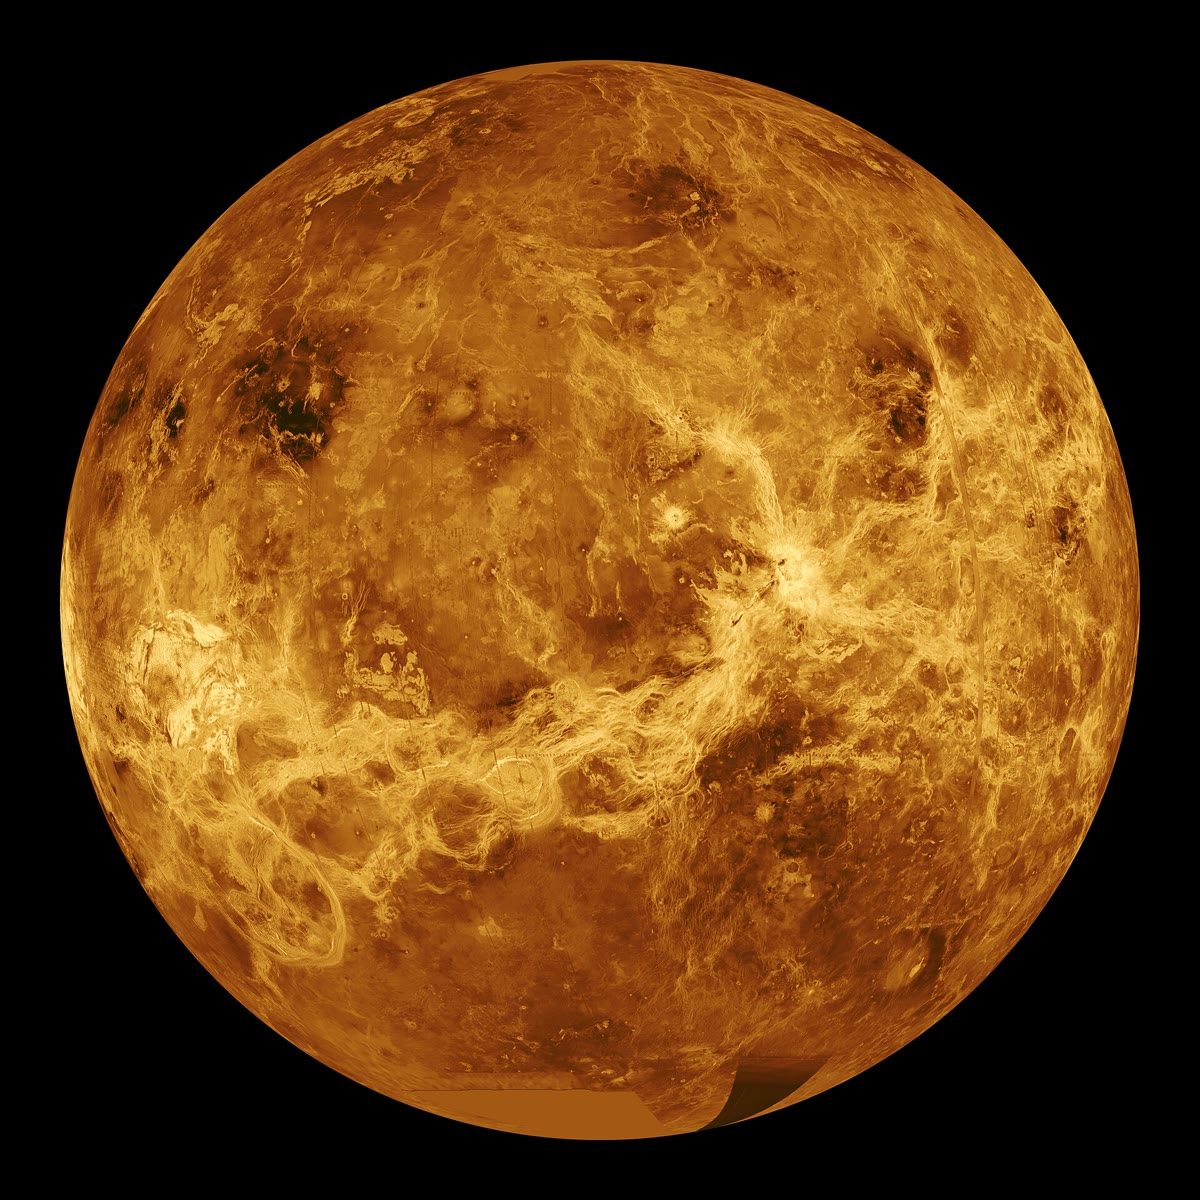
\includegraphics[width=\linewidth]{images/book3/b1-venus-radar-globe.jpg}
\end{minipage}\hspace{0.06\linewidth}
\begin{minipage}{0.4\linewidth}
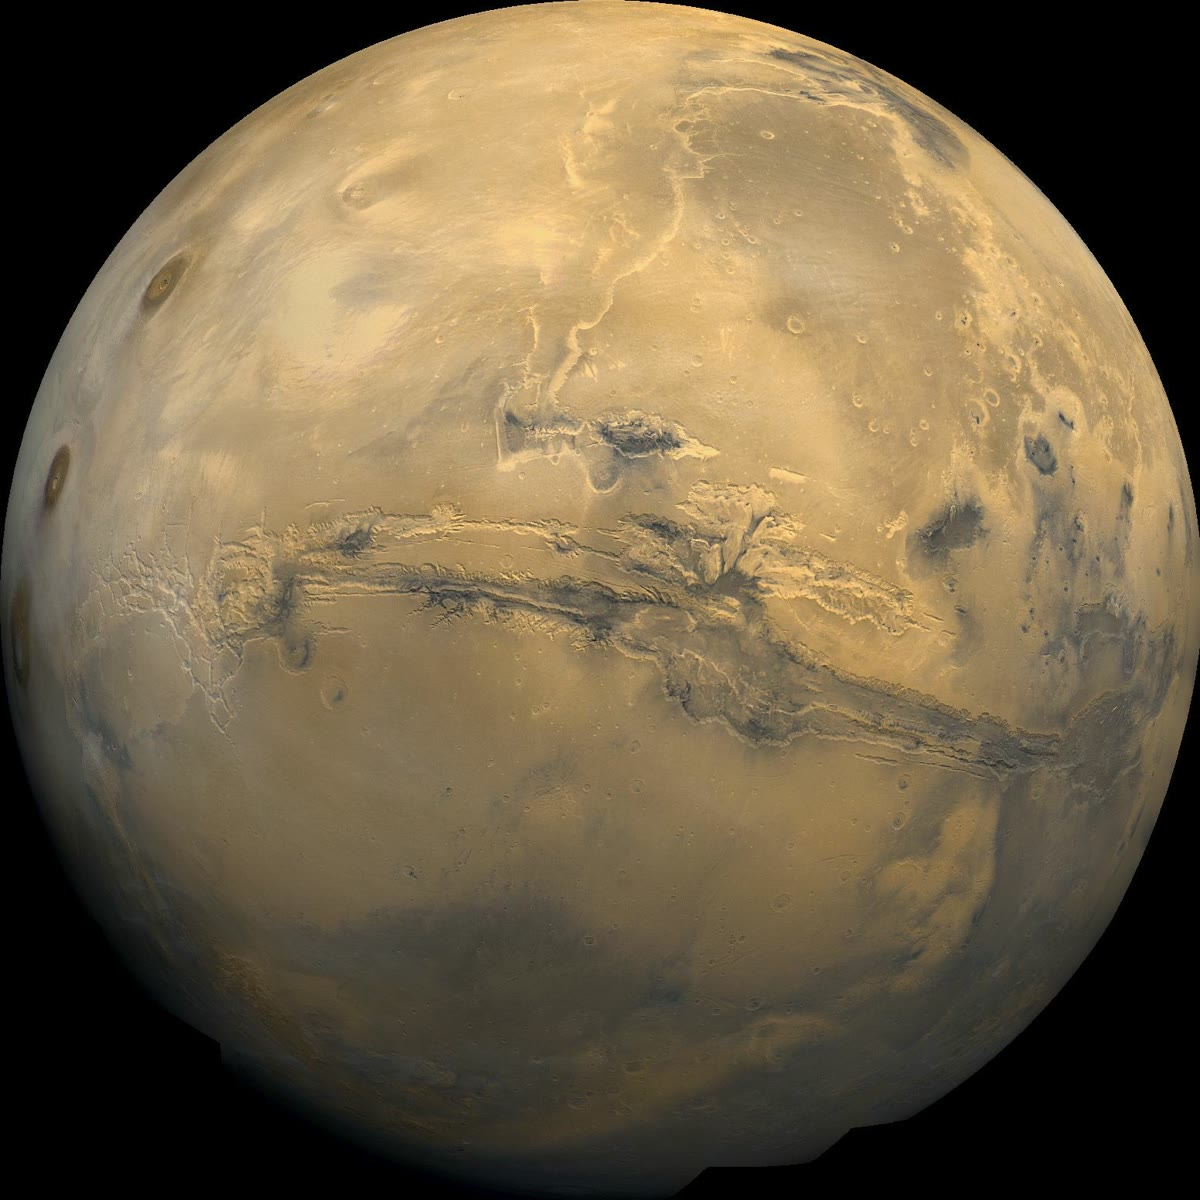
\includegraphics[width=\linewidth]{images/book3/b1-mars-valles-marineris.jpg}
\end{minipage}

{\small A la izquierda: la superficie de Venus vista a través de sus nubes por el radar de la
nave Magallanes, cartografiada sobre un globo simulado por ordenador (los colores son
simulados). A la derecha: Marte, desde el orbitador Viking 1, un mosaico centrado en el sistema
de cañones de Valles Marineris. NASA/JPL y NASA/USGS, dominio público.}
% ledger: commons:venus-globe, commons:mars-valles
\end{omfigure}

La superficie conserva el registro de lo que la moldeó. Los cráteres de impacto se acumulan sobre
cualquier superficie expuesta al espacio; así, una superficie muy cráterizada, como la mayor parte
de la de la Luna o de Mercurio, es antigua, y una superficie con pocos cráteres ha sido renovada:
por coladas de lava, por erosión o por las placas que devuelven el fondo oceánico terrestre al
manto. Llanuras volcánicas y volcanes se encuentran en todos los \omterm{def:b1:comparative-planetology:planet-types}{planetas terrestres}. Fallas,
grietas y cinturones plegados muestran que las litosferas de Venus y de Marte se han deformado;
pero de todos los planetas, solo la Tierra muestra hoy una litosfera dividida en placas que se
mueven como bloques rígidos, con dorsales donde se forman y fosas donde se hunden. Por qué solo
la Tierra tiene tectónica de placas sigue discutiéndose; la presencia de agua, que debilita las
rocas, es una de las razones propuestas.

\section{Lunas y cuerpos pequeños}

La Luna, con un cuarto del diámetro terrestre, es grande para un satélite. Su densidad,
\qty{3340}{kg.m^{-3}}, parecida a la de las rocas del manto terrestre, y su \omterm{def:b1:comparative-planetology:moi}{factor de momento de
inercia}, cercano a $0.4$, muestran que tiene a lo sumo un pequeño núcleo de hierro. Los \omterm{def:b1:comparative-planetology:planet-types}{planetas
gigantes} tienen sistemas de lunas que son mundos en sí mismos (véanse las fotografías siguientes).
Ío, la más interior de las cuatro grandes lunas de Júpiter, es el mundo más activo volcánicamente
del sistema solar, con cientos de volcanes, calentado por las mareas que Júpiter levanta en él;
el vulcanismo la renueva más deprisa de lo que los impactos pueden marcarla con grandes cráteres.
Europa, de densidad \qty{3010}{kg.m^{-3}}, es roca bajo una corteza de hielo, y hay pruebas
sólidas de un océano salado bajo esa corteza. Ganímedes y Calisto, con densidades de \num{1940} y
\qty{1830}{kg.m^{-3}}, están hechas de roca y hielo en cantidades comparables.
Titán, la mayor luna de Saturno, es la única luna con una atmósfera densa, sobre todo de
nitrógeno con un poco de metano, y el único mundo, aparte de la Tierra, con ríos, lagos y mares
en su superficie —de metano y etano líquidos—; probablemente también esconde un océano de agua.
% ledger: planet:Moon.diameter, planet:Earth.diameter, planet:Moon.density, nasa:moon, nasa:io-facts, nasa:europa, nasa:europa-facts, nasa:ganymede, nasa:titan-facts

\begin{omfigure}
\begin{minipage}{0.4\linewidth}
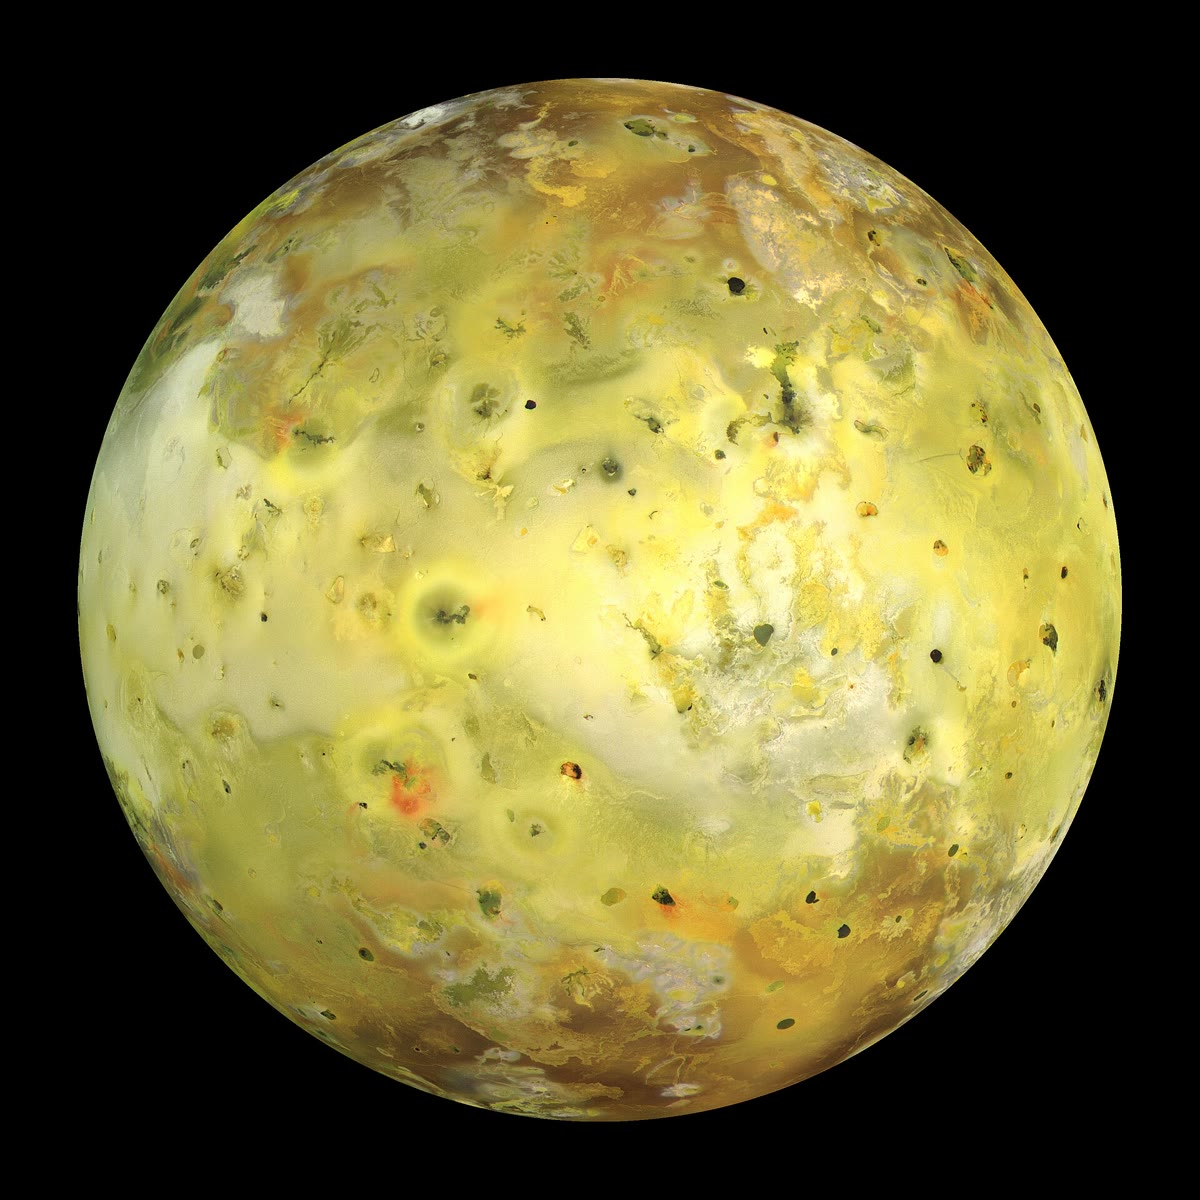
\includegraphics[width=\linewidth]{images/book3/b1-io.jpg}
\end{minipage}\hspace{0.06\linewidth}
\begin{minipage}{0.4\linewidth}
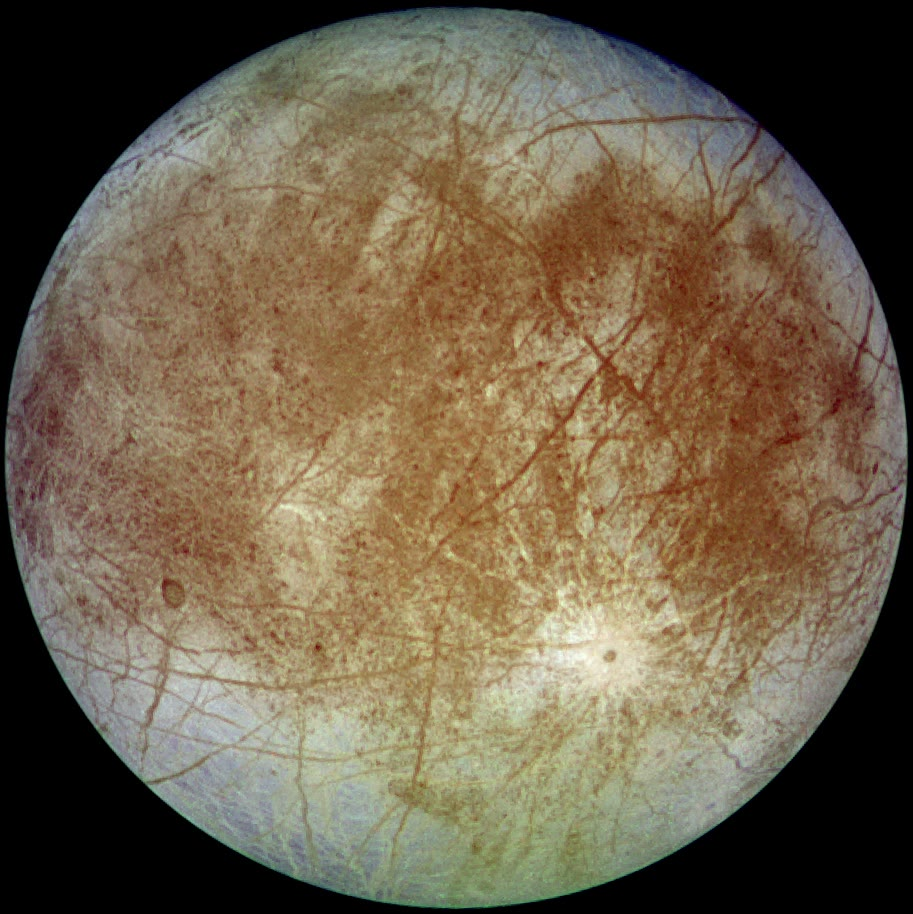
\includegraphics[width=\linewidth]{images/book3/b1-europa.jpg}
\end{minipage}

{\small Dos de las grandes lunas de Júpiter vistas por la nave Galileo. A la izquierda: Ío, con
su superficie salpicada de centros volcánicos y coloreada por compuestos de azufre y lavas. A la
derecha: Europa en color natural aproximado; las largas líneas oscuras son fracturas de su
corteza de hielo. NASA/JPL/University of Arizona y NASA/JPL/DLR, dominio público.}
% ledger: commons:io, commons:europa, nasa:io-facts, nasa:europa
\end{omfigure}

\begin{definition}[Asteroide, cometa, objeto transneptuniano]\label{def:b1:comparative-planetology:small-bodies}
Un \emph{asteroide}\index{asteroide} es un cuerpo pequeño, rocoso o metálico, que orbita el Sol,
demasiado pequeño para ser un planeta y sin la envoltura de gas y polvo de un cometa; la mayoría
orbita entre Marte y Júpiter. Un \emph{cometa}\index{cometa} es un cuerpo pequeño de hielo y
polvo que, cuando su órbita lo acerca al Sol, libera gas y polvo que forman a su alrededor una
envoltura luminosa y colas que apuntan en dirección opuesta al Sol. Un \emph{objeto
transneptuniano}\index{objeto transneptuniano} es un cuerpo del sistema solar cuya órbita está,
en promedio, más allá de la de Neptuno.
\end{definition}

Los \omterm{def:b1:comparative-planetology:small-bodies}{objetos transneptunianos} del cinturón de Kuiper, una zona en forma de disco más allá de
Neptuno, son cuerpos de hielo y roca que quedaron de la formación de los planetas; Plutón,
clasificado como planeta enano desde 2006, es uno de ellos. Los \omterm{def:b1:comparative-planetology:small-bodies}{asteroides} son los restos de una
región donde no se formó ningún planeta. Fragmentos de \omterm{def:b1:comparative-planetology:small-bodies}{asteroides}, y algunos de la Luna y de Marte,
caen sobre la Tierra como meteoritos. Son las únicas muestras de otros mundos que tenemos en la
mano, aparte de las traídas por naves espaciales, y algunos han cambiado poco desde que se formó
el sistema solar; sus clases, y lo que dicen sobre la composición de la Tierra y la edad del sistema
solar, son el tema del libro 4, segundo año.
% ledger: nasa:pluto-facts

\section{Ejercicios}

\begin{exercise}[$\star$]\label{exo:b1:comparative-planetology:1}
Júpiter tiene una masa de \qty{1898.13e24}{kg} y un radio medio de \qty{69911}{km}. Calcúlese
su densidad media y compárese con la del agua, \qty{1000}{kg.m^{-3}}.
\end{exercise}

\begin{exercise}[$\star$]\label{exo:b1:comparative-planetology:2}
Con la figura de densidades y radios, clasifíquense Mercurio, Saturno, Urano y Venus como
\omterm{def:b1:comparative-planetology:planet-types}{planetas terrestres}, \omterm{def:b1:comparative-planetology:planet-types}{gigantes gaseosos} o \omterm{def:b1:comparative-planetology:planet-types}{gigantes de hielo}, y justifíquese cada elección por su
radio y su densidad.
\end{exercise}

\begin{exercise}[$\star$]\label{exo:b1:comparative-planetology:3}
Venus recibe \qty{2601.3}{W.m^{-2}} y tiene un \omterm{def:b1:comparative-planetology:albedo}{albedo de Bond} de 0.77. Calcúlese su \omterm{def:b1:comparative-planetology:equilibrium-temperature}{temperatura
de equilibrio}. ¿Por qué es más baja que la de la Tierra, aunque Venus esté más cerca del Sol?
\end{exercise}

\begin{exercise}[$\star$]\label{exo:b1:comparative-planetology:4}
Ordénense la Luna ($C = 0.394$), Marte (0.366), la Tierra (0.3308), Júpiter (0.254) y Saturno
(0.210) de la más uniforme a la más concentrada en el centro. ¿Cuál sería $C$ para un planeta
cuya masa entera estuviera en un punto de su centro?
\end{exercise}

\begin{exercise}[$\star\star$]\label{exo:b1:comparative-planetology:5}
Titán orbita Saturno a $a = \qty{1221.87e3}{km}$ en \num{15.945421} días. Calcúlese la masa de
Saturno y compárese con el valor tabulado, \qty{568.32e24}{kg}.
\end{exercise}

\begin{exercise}[$\star\star$]\label{exo:b1:comparative-planetology:6}
La Tierra recibe \qty{1361}{W.m^{-2}} a \qty{149.6e6}{km} del Sol. Calcúlese la irradiancia en
Marte (\qty{228.0e6}{km}) y en Júpiter (\qty{778.5e6}{km}), y compárese con los valores tabulados
\qty{586.2}{W.m^{-2}} y \qty{50.26}{W.m^{-2}}.
\end{exercise}

\begin{exercise}[$\star\star$]\label{exo:b1:comparative-planetology:7}
Demuéstrese que, para un albedo dado, $T_\mathrm{eq}$ varía como $d^{-1/2}$. Calcúlese
$T_\mathrm{eq}$ para Júpiter ($S = \qty{50.26}{W.m^{-2}}$, $A = 0.343$). Si se observara que
Júpiter radia más potencia de la que absorbe del Sol, ¿qué implicaría eso sobre su interior?
\end{exercise}

\begin{exercise}[$\star\star$]\label{exo:b1:comparative-planetology:8}
Calcúlese el calentamiento por efecto invernadero $T_\mathrm{surf} - T_\mathrm{eq}$ de Venus
(\qty{737}{K}), de la Tierra (\qty{288}{K}, $A = 0.294$) y de Marte (\qty{214}{K}). Exprésese
cada uno como fracción de $T_\mathrm{eq}$.
\end{exercise}

\begin{exercise}[$\star\star$]\label{exo:b1:comparative-planetology:9}
Para una esfera uniforme, demuéstrese que $C = 0.4$ integrando los momentos de inercia de
capas esféricas delgadas (una capa de radio $r$ y masa $\mathrm dm$ tiene
$\mathrm dI = \tfrac23 r^2\,\mathrm dm$). ¿Qué valor tiene una capa esférica hueca de radio $R$?
\end{exercise}

\begin{exercise}[$\star\star\star$]\label{exo:b1:comparative-planetology:10}
Mercurio tiene $\bar\rho = \qty{5429}{kg.m^{-3}}$, $C = 0.35$ y un radio de \qty{2439.7}{km}.
Con una densidad del manto de \qty{3300}{kg.m^{-3}}, úsese el modelo de dos capas para hallar el
radio de su núcleo, la densidad del núcleo y la fracción de su masa que está en el núcleo.
¿Qué tiene de notable Mercurio?
\end{exercise}

\begin{exercise}[$\star\star\star$]\label{exo:b1:comparative-planetology:11}
Modélese un cuerpo sin atmósfera cuyo hemisferio diurno está a la temperatura uniforme $T_1$ y
el nocturno a $T_2$, radiando juntos la potencia absorbida. (a) Demuéstrese que si
$T_1^4 + T_2^4 = 2T_\mathrm{eq}^4$, la temperatura media $(T_1 + T_2)/2$ es como mucho
$T_\mathrm{eq}$, con igualdad solo cuando $T_1 = T_2$. (b) Para la Luna, $T_\mathrm{eq} = \qty{270}{K}$; tómese $T_2 = \qty{100}{K}$. Calcúlense $T_1$ y la temperatura media.
\end{exercise}

\begin{exercise}[$\star\star\star$]\label{exo:b1:comparative-planetology:12}
Venus tiene un radio de \qty{6051.8}{km}, una gravedad superficial de \qty{8.9}{m.s^{-2}} y una
presión superficial de \qty{92}{bar}. Calcúlese la masa de su atmósfera, compárese con la de la
Tierra, \qty{5.1e18}{kg}, y con la masa de Venus, \qty{4.8673e24}{kg}. ¿Qué sugiere la
comparación sobre dónde se guarda el dióxido de carbono de la Tierra?
% ledger: earth:Matm, planet:Venus.gravity, nasa:venus
\end{exercise}

\section{Problema: pesar y sondear Marte}

\begin{problem}[{Problema de fin de semana --- la masa de Marte a partir de su luna, su densidad
y su temperatura, y el tamaño de su núcleo}]
\label{pb:b1:comparative-planetology:1}
% ledger: nasa:phobos, nasa:mars, nasa:mars-core, const:G, const:sigma, earth:psurf, earth:gmean, planet:Mars.Prot, planet:Earth.density
% numbers computed in the scratch calculator calc/ch03.py from the rounded data
Fobos, la mayor de las lunas de Marte, orbita a una distancia media de \qty{9378}{km} del centro
de Marte en \num{0.31891} días. Marte tiene un radio medio de \qty{3389.5}{km}, un periodo de
rotación de \qty{24.6}{h}, un \omterm{def:b1:comparative-planetology:moi}{factor de momento de inercia} $C = 0.366$, un \omterm{def:b1:comparative-planetology:albedo}{albedo de Bond} de 0.250
y una presión superficial media de \qty{6.36}{mbar}; recibe \qty{586.2}{W.m^{-2}} del Sol, y su
temperatura superficial media es de unos \qty{214}{K}. Fobos tiene una masa de \qty{1.06e16}{kg}.
Tómese $G = \qty{6.6743e-11}{m^3.kg^{-1}.s^{-2}}$ y $\sigma = \qty{5.6704e-8}{W.m^{-2}.K^{-4}}$.

\medskip
\noindent\textbf{Parte I --- Pesar Marte.}
\begin{enumerate}
  \item Conviértase el periodo de Fobos a segundos.
  \item Calcúlese $GM$ para Marte.
  \item Dedúzcase la masa de Marte.
  \item ¿Es correcto despreciar la masa de Fobos?
  \item Calcúlese la velocidad orbital de Fobos.
  \item Compárese el periodo de Fobos con la rotación de Marte. ¿En qué sentido cruza Fobos el
        cielo de Marte?
\end{enumerate}

\medskip
\noindent\textbf{Parte II --- Densidad y gravedad.}
\begin{enumerate}[resume]
  \item Calcúlese el volumen de Marte.
  \item Calcúlese su densidad media, redondeada a \qty{10}{kg.m^{-3}}.
  \item Compárese con la de la Tierra, \qty{5514}{kg.m^{-3}}. Dense dos razones por las que la
        Tierra es más densa.
  \item Calcúlese la gravedad en la superficie de Marte.
  \item Calcúlese la velocidad de escape desde la superficie de Marte.
\end{enumerate}

\medskip
\noindent\textbf{Parte III --- Temperatura y atmósfera.}
\begin{enumerate}[resume]
  \item Calcúlese la \omterm{def:b1:comparative-planetology:equilibrium-temperature}{temperatura de equilibrio} de Marte.
  \item Compárese con la temperatura superficial media. ¿Cuánto vale el calentamiento por efecto
        invernadero?
  \item Calcúlese la masa de la atmósfera sobre cada metro cuadrado de Marte, y compárese con la de
        la Tierra ($p = \qty{1014}{hPa}$, $g = \qty{9.82}{m.s^{-2}}$).
  \item Calcúlese la masa total de la atmósfera de Marte.
  \item La atmósfera de Marte es un \qty{95}{\percent} de dióxido de carbono, y sin embargo su
        calentamiento por efecto invernadero es pequeño. Sugiérase por qué.
\end{enumerate}

\medskip
\noindent\textbf{Parte IV --- El núcleo de Marte.}
\begin{enumerate}[resume]
  \item ¿Cuál sería $C$ si Marte fuera uniforme? ¿Qué indica el valor medido?
  \item Escríbase la densidad media de un Marte de dos capas en función del radio relativo del
        núcleo $x$, de la densidad del manto $\rho_m$ y de la densidad del núcleo $\rho_c$.
  \item Escríbase su \omterm{def:b1:comparative-planetology:moi}{factor de momento de inercia} en los mismos términos.
  \item Demuéstrese que $x^2 = (\tfrac52C\bar\rho - \rho_m)/(\bar\rho - \rho_m)$.
  \item Con la densidad media de la pregunta 8 y $\rho_m =
        \qty{3500}{kg.m^{-3}}$, calcúlense $x$ y la densidad del núcleo.
  \item ¿Qué fracción de la masa de Marte está en su núcleo?
  \item Repítase la pregunta 21 con $\rho_m = 3450$ y \qty{3550}{kg.m^{-3}}. ¿Qué concluye
        sobre la precisión del modelo?
  \item Dése el radio del núcleo de Marte según el modelo con $\rho_m = \qty{3500}{kg.m^{-3}}$, y
        compárese con el valor de la tabla planetaria, \qty{1830}{km}, y con el resultado sísmico
        reciente, de \qty{1650}{km} a \qty{1675}{km}.
\end{enumerate}
\end{problem}
